\documentclass[11pt]{article} % use larger type; default would be 10pt
\usepackage{mathrsfs,amsmath}
\usepackage{gensymb}
\usepackage{graphicx}
\usepackage{float}
\graphicspath{ {images/} }
\usepackage{fixltx2e} %for subscript
\usepackage[margin=0.8in]{geometry}
\setlength{\parskip}{\baselineskip}%
\setlength{\voffset}{0in}
%\pagenumbering{gobble}

\title{Testing the 1D SCFT code}
%\author{Rui Xu}
\date{} % Activate to display a given date or no date (if empty),
         % otherwise the current date is printed 
         
\begin{document}

\large Testing the 1D SCFT code

\section{Introduction}

I constructed a code that would allow for the calculation of equilibrium structures and their free energies in 1 dimension, with planar, cylindrical, and spherical geometries. This code will be used to calculate various bending moduli to determine the Helfrich free energy of two types of membranes - an AB-diblock copolymer bilayer membrane in C-homopolymer and an ABA-triblock copolymer monolayer membrane in C-homopolymer. Once a comparison between these membranes is finished, we will investigate blends of AB-diblock copolymers with ABA-triblock copolymers.

\section{Convergence of Coordinate systems}
\subsection{AB-diblock system}

The first test performed was to determine if the free energies of the three codes agree when taking the limit of large cylinder and large sphere radii and comparing them to the free energy of the cartesian system. We use lamellar structures for this calculation, and use a Flory-Huggins interaction parameter $\chi_{AB}=20$, and a box size of 4$R_g$. We expect that the free energy at small radii will be larger for spherical and cylindrical systems due to the increased curvature of the computational box, which increases the bending energy(?) or reduces configurational entropy(?). The free energy of the lamella in cylindrical and spherical systems, relative to the Cartesian system, is shown in Figure 1.

\begin{figure}[H]
\centering
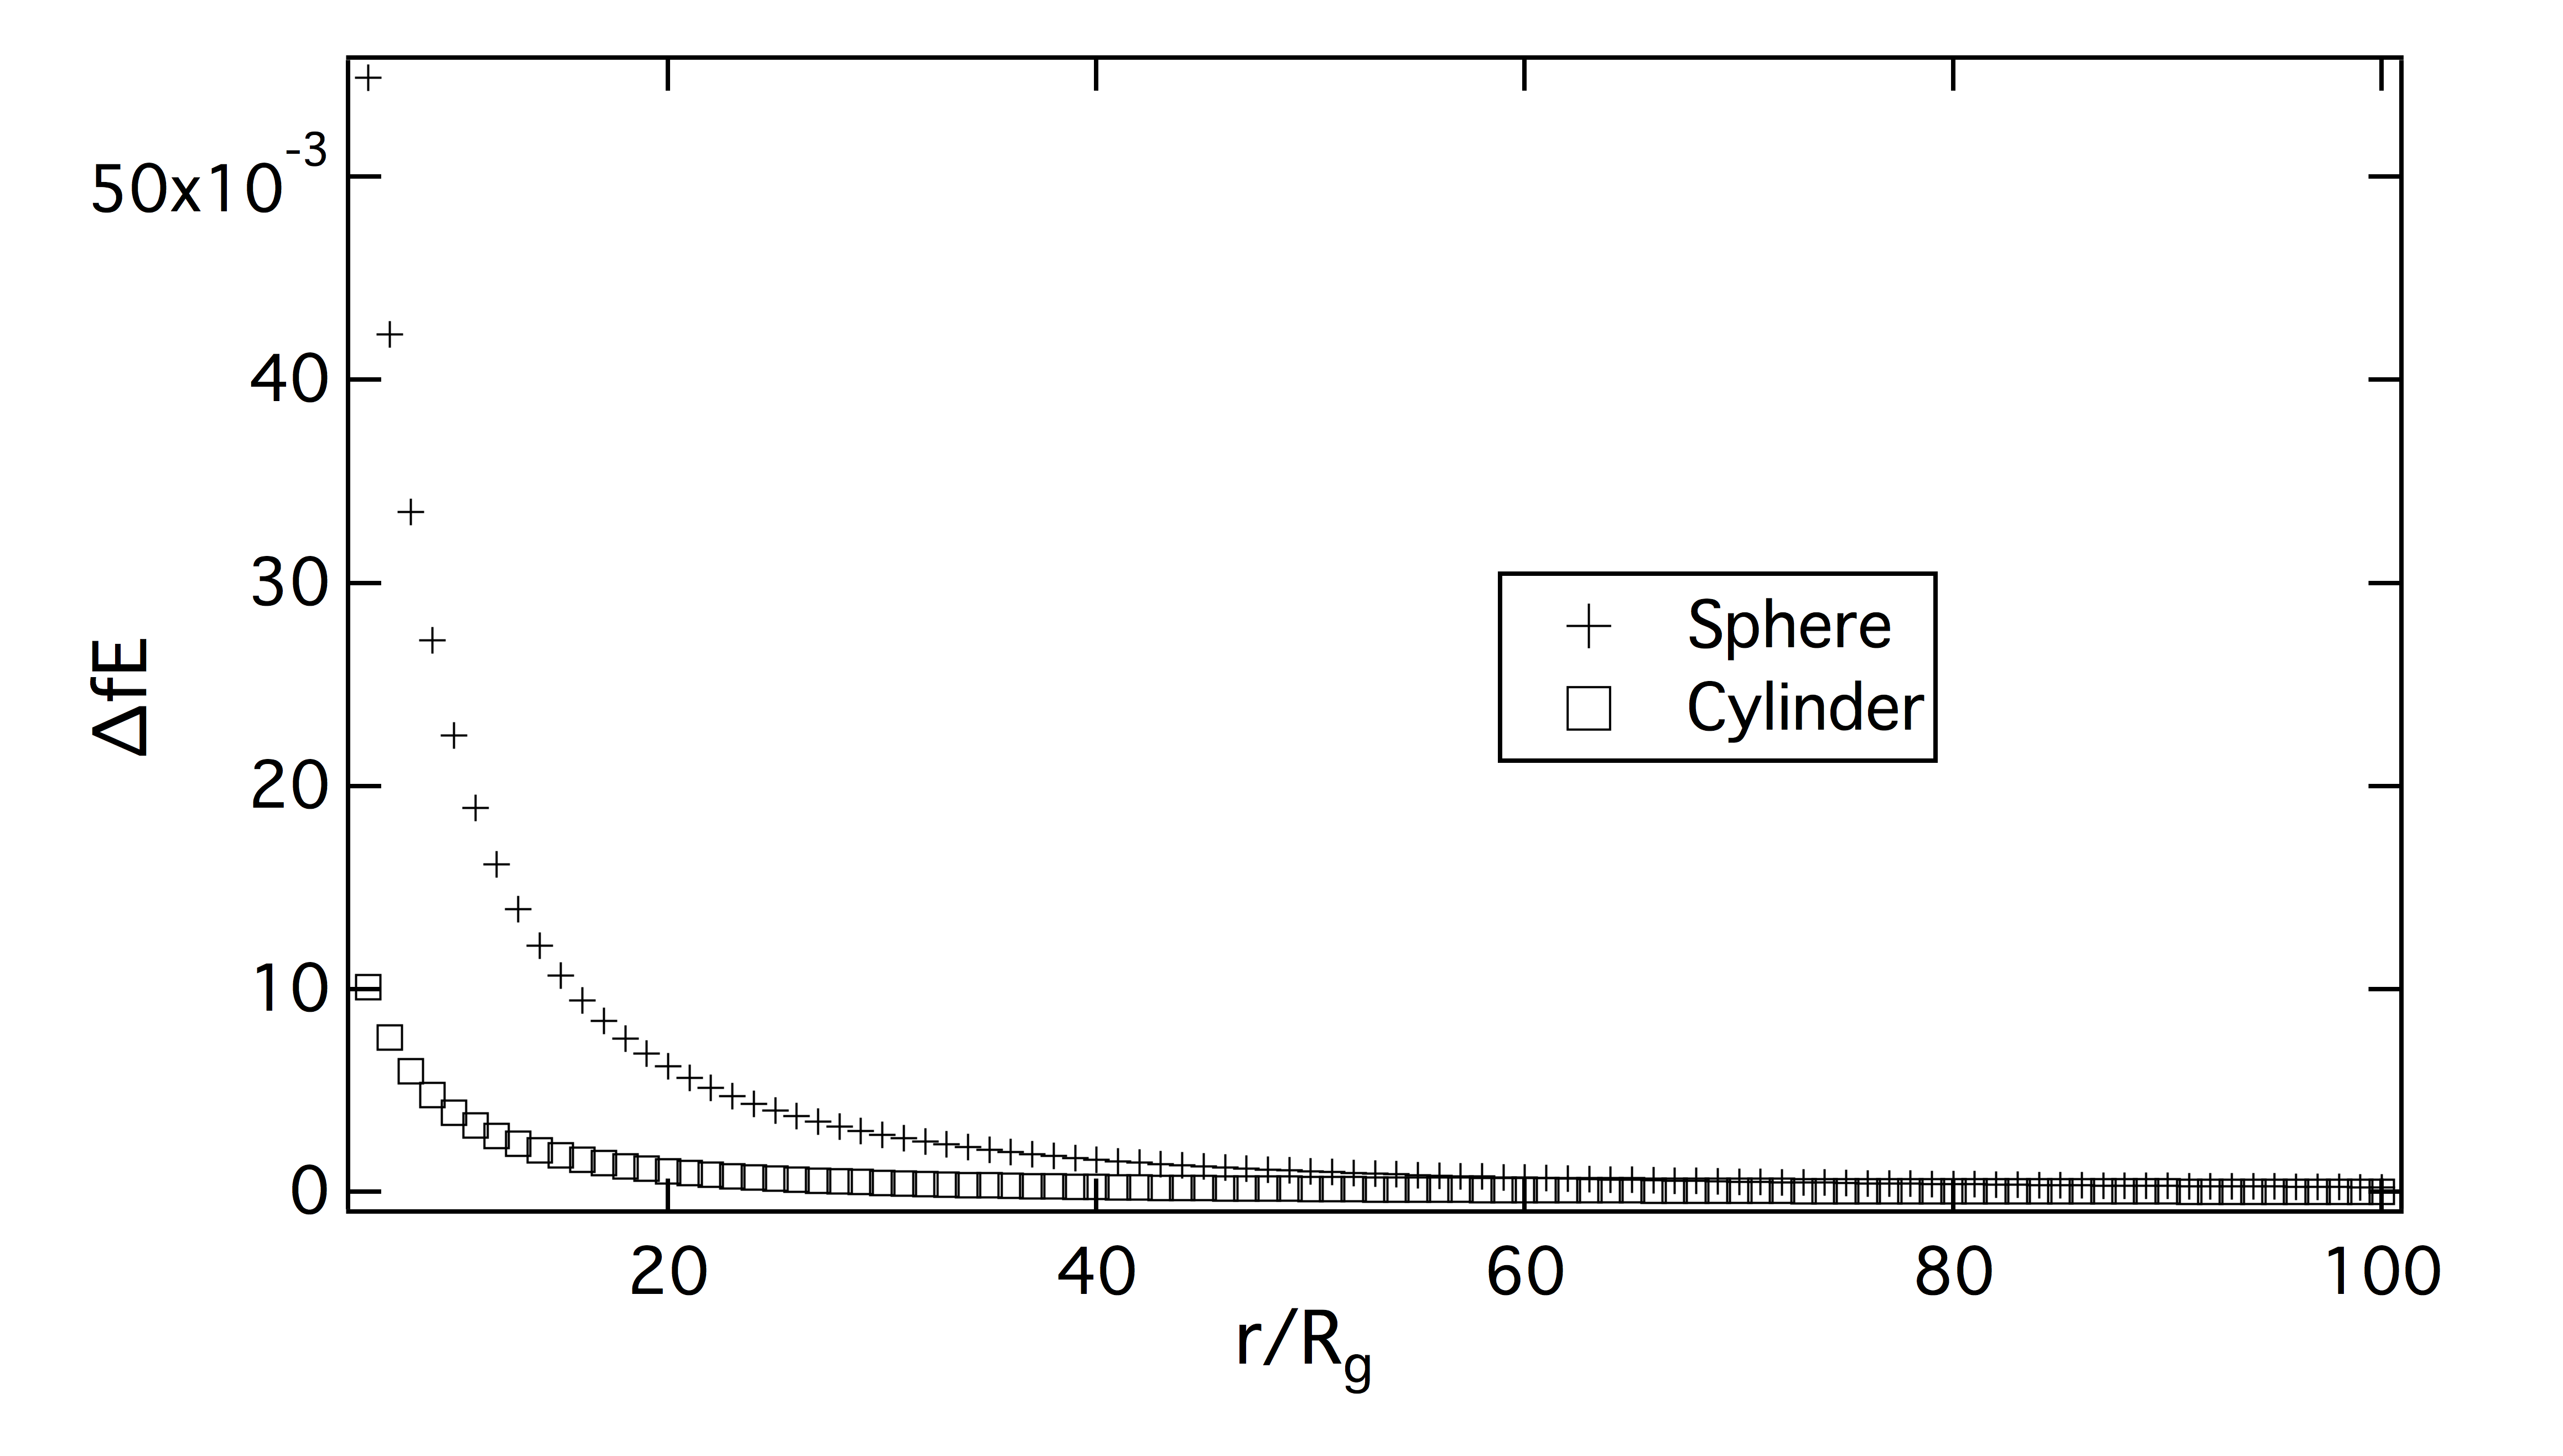
\includegraphics[scale=0.5]{rad_conv2}
\caption{Difference in free energy between AB diblock copolymer lamella in cylindrical and spherical geometries relative to the planar geometry for different cylinder and sphere radii.}
\centering
\end{figure}
\noindent
Figure 1 shows that in the limit of large radii, the free energy of the lamella in the cylindrical and spherical systems approaches that of the lamella in Cartesian coordinates. This is good, and is the expected relationship.

\subsection{ABA-triblock system}

The ABA-triblock system was tested, with the same expectations as the AB-diblock system. The results are shown in Figure 2.

\begin{figure}[H]
\centering
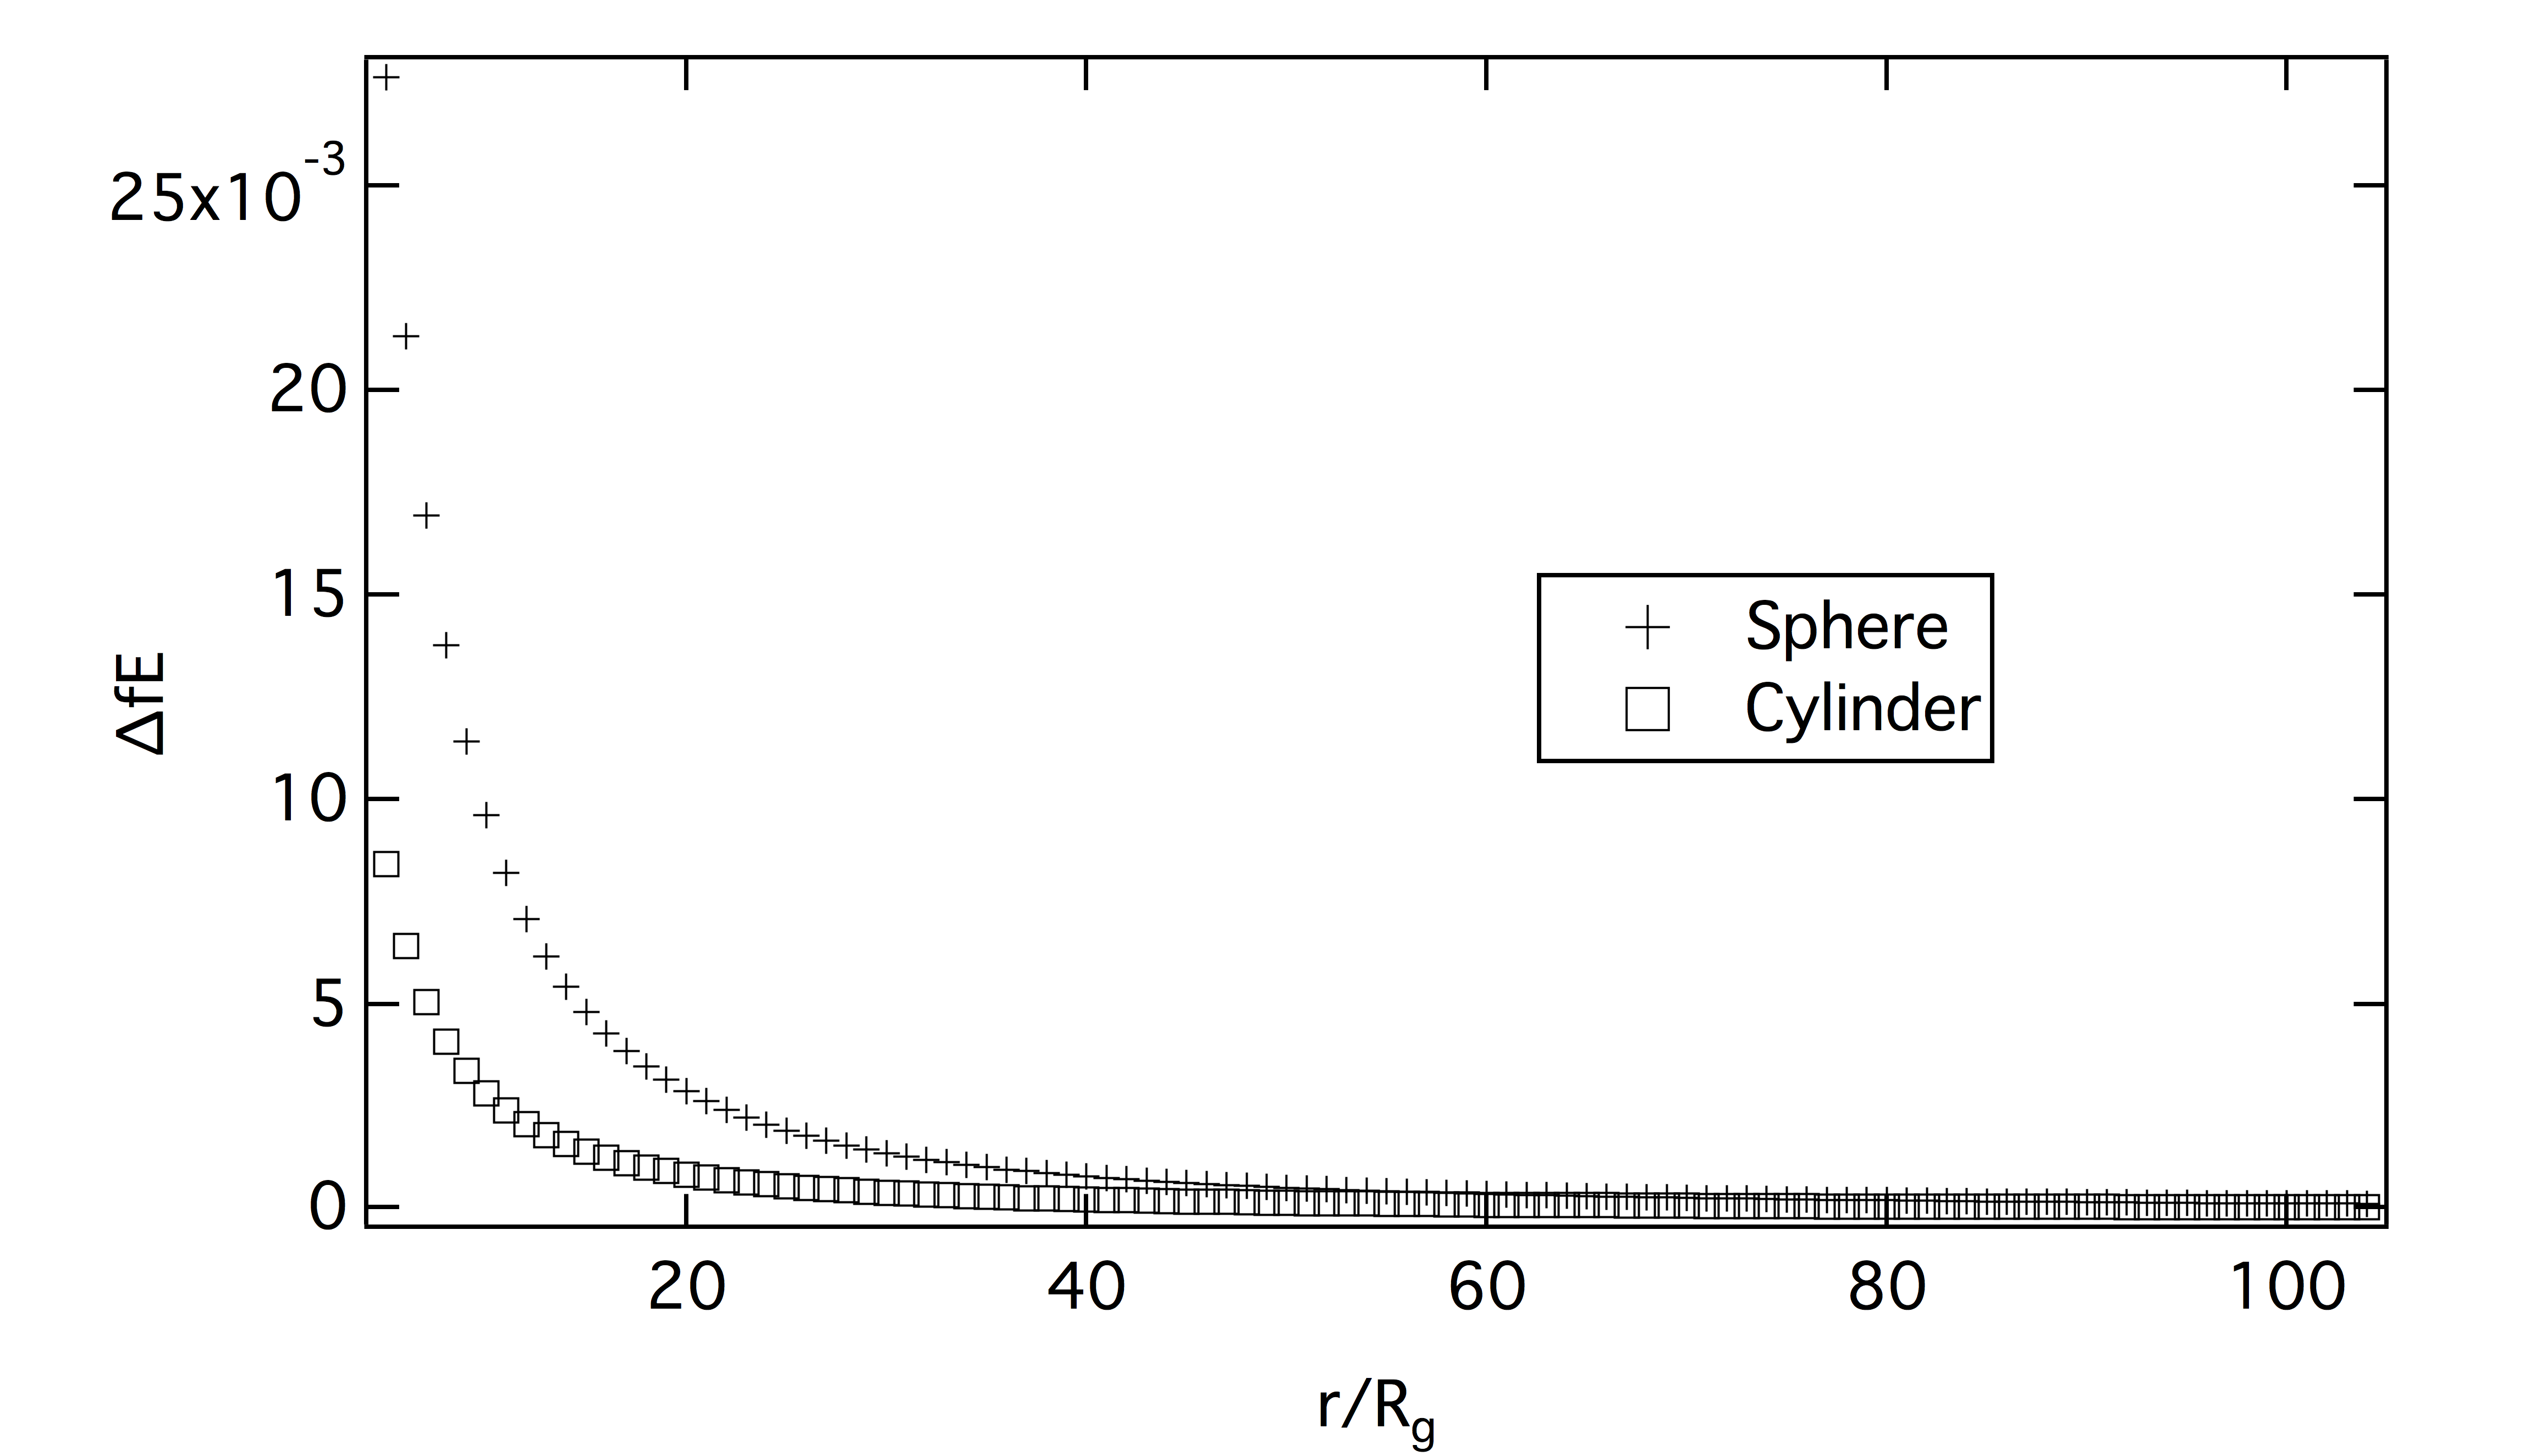
\includegraphics[scale=0.5]{rad_conv3}
\caption{Difference in free energy between ABA triblock copolymer lamella in cylindrical and spherical geometries relative to the planar geometry for different cylinder and sphere radii.}
\centering
\end{figure}

The results for the ABA-triblock system are not exactly the same as for the AB-diblock system. The difference between cylindrical geometry and planar geometry are similar for the two systems, but there is a fairly large difference between the spherical geometries. I'm not sure if this is correct, or if there could be a problem with my free energy calculation. To be investigated. 


\section{The membrane - lipid concentration profile}
\subsection{AB-diblock copolymer bilayer membrane - Spherical coordinates}

The initial $\omega$ auxiliary field was changed from the cosines used to create the lamellar system to an initial condition intended to create a bilayer. The chemical potential of the AB-diblock was set to zero, the chemical potential of the ABA-triblock was set to -20 to push it out of the system, and the chemical potential of the $C$ homopolymer was set to -3.906, previously determined to be the chemical potential of a tensionless bilayer. Box size was set to 12 $R_g$ to allow the system to reach bulk concentrations at the edges, and the distance from the innermost edge of the box from the centre of the sphere was set to 4$R_g$ such that the bilayer was centered at approximately $10R_g$ from the centre of the coordinate system. Free energy was calculated (less than -1.0, not sure if right), and the concentration profile was calculated. The resulting concentration profile is shown in Figure XX.

\begin{figure}[H]
\centering
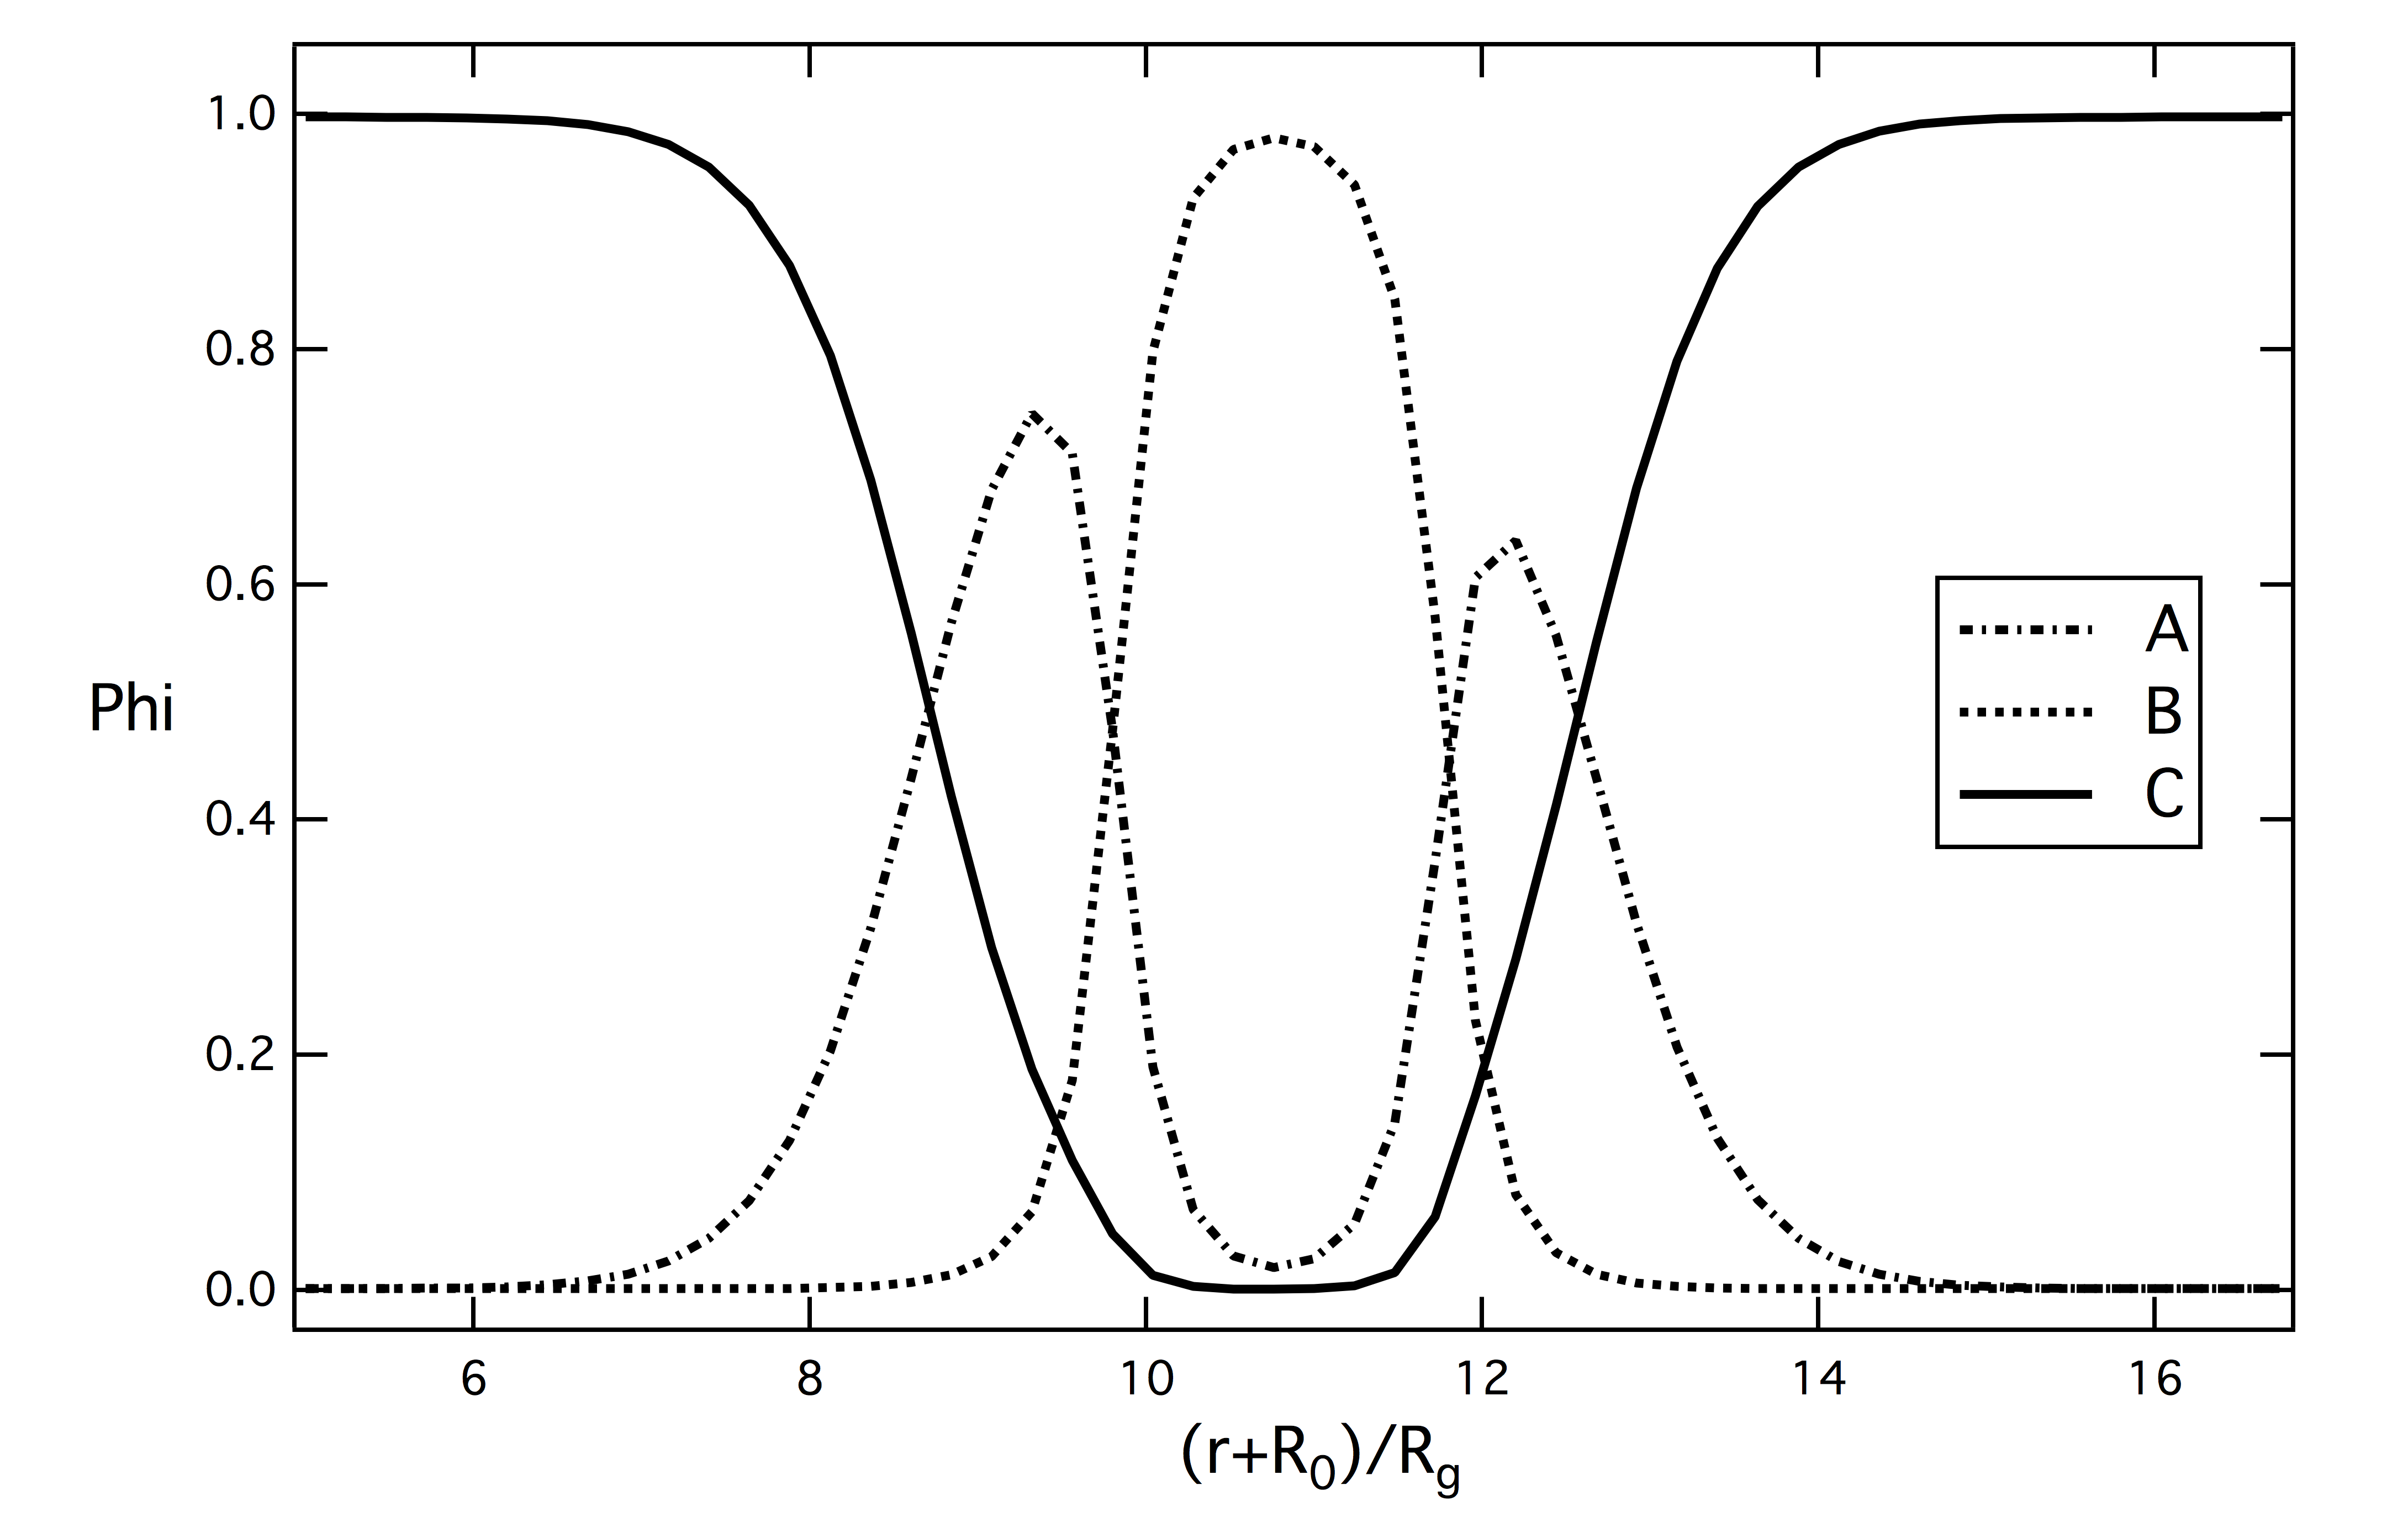
\includegraphics[scale=0.6]{bilayer_AB}
\centering
\end{figure}

\subsection{ABA-triblock copolymer monolayer membrane - Spherical coordinates}

The same calculation with different initial chemical potentials was used to determine the concentration profile for the ABA-triblock copolymer membrane. In this case, the chemical potential of the AB-diblock copolymer was set to -20, the chemical potential of the ABA-triblock copolymer was set to zero, and once again the chemical potential of the homopolymer was set to -3.906. The concentration profile is shown in Figure XX.

Note, the chemical potential for a tensionless membrane isn't -3.906 in this code, so the membrane shown in this diagram is not fully tensionless.However, these diagrams were solely used to show that the concentration profiles of the two systems were of the expected form.
\begin{figure}[H]
\centering
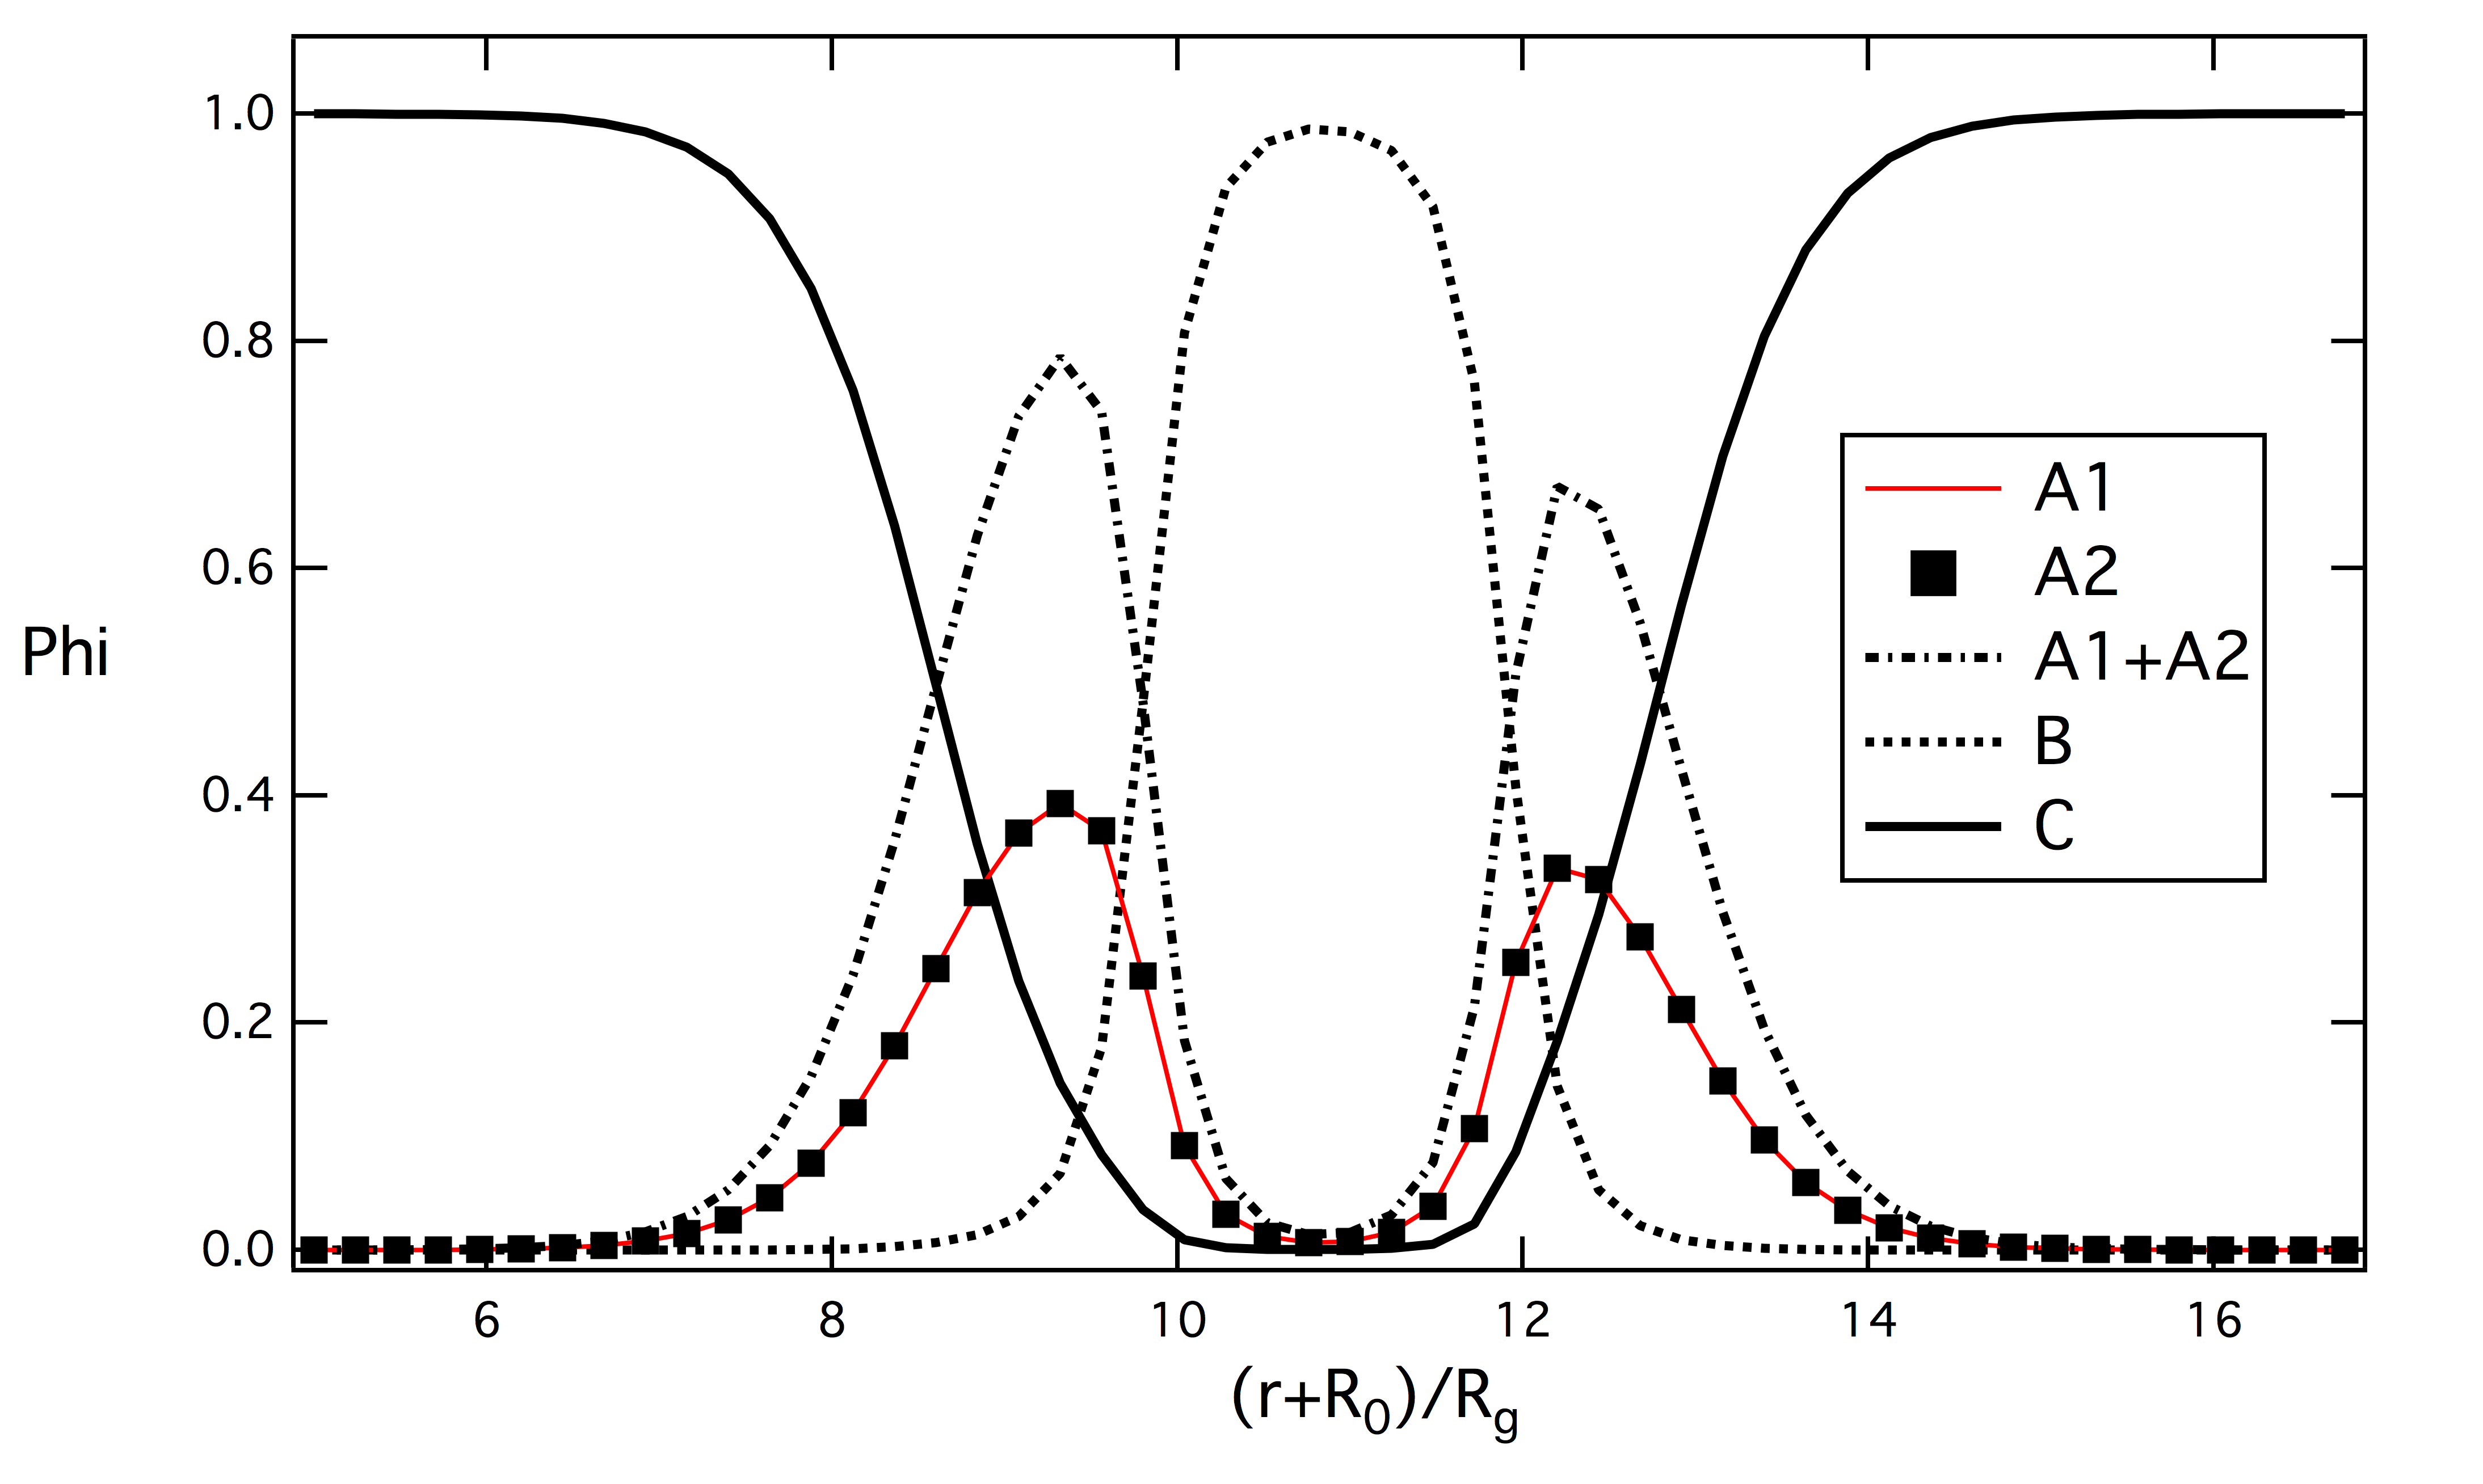
\includegraphics[scale=0.6]{monolayer_ABA}
\centering
\end{figure}

Note, the chemical potential for a tensionless membrane isn't -3.906 in this code, so the membrane shown in this diagram is not fully tensionless.However, these diagrams were solely used to show that the concentration profiles of the two systems were of the expected form.
\section{Bending moduli}

\subsection{Tensionless Bilayer}

We determine the chemical potential for a tensionless membrane using the planar coordinate system. This chemical potential is found where the free energy of the membrane system is equal to the free energy of a homogeneous system. For the ABA-triblock copolymer system, the relative chemical potential of the $C$-homopolymer for a tensionless membrane wwas determined to be -5.248. For the AB-diblock copolymer system, the relative chemical potential of the $C$-homopolymer for a tensionless membrane was determined to be -5.338.I'm not sure if the difference in chemical potentials between the two systems should be there, but that's what the code is telling me at the moment. The homogeneous free energy densities of the two systems are the same, so there isn't a problem in that function.

\noindent
Next, the free energies for bilayers of small to large radii (large to small curvatures) were calculated for spherical and cylindrical geometries. We define curvature $c$ as the average membrane width ($ d = 4.3 R_g$) divided by the radius of the membrane, measured from the centre of the membrane to the centre of the spherical or cylindrical coordinate system. 

\begin{equation}
C=d/r
\end{equation}

\subsection{Bending Moduli}

In cylindrical geometry, the calculated free energy ($F^C$) originates from the mean curvature contribution to the Helfrich bending energy, while the Gaussian curvature contribution is zero. Ignoring higher order bending moduli (?), the free energy is a function of curvature:

\begin{equation}
F^C = \frac{\kappa_M}{2} C^2
\end{equation}

\noindent
In spherical geometry, the calculated free energy ($F^S$) originates from both mean curvature and Gaussian curvature contributions. Ignoring higher order bending moduli, the free energy is again expressed as a function of curvature.

\begin{equation}
F^S = (2 \kappa_M + \kappa_G)C^2
\end{equation}

I calculated free energy for a range of curvatures (range can be extended in some cases, but it was hard to stabilize bilayer at very high curvatures). The results are shown in Figure XX.

\begin{figure}[H]
\centering
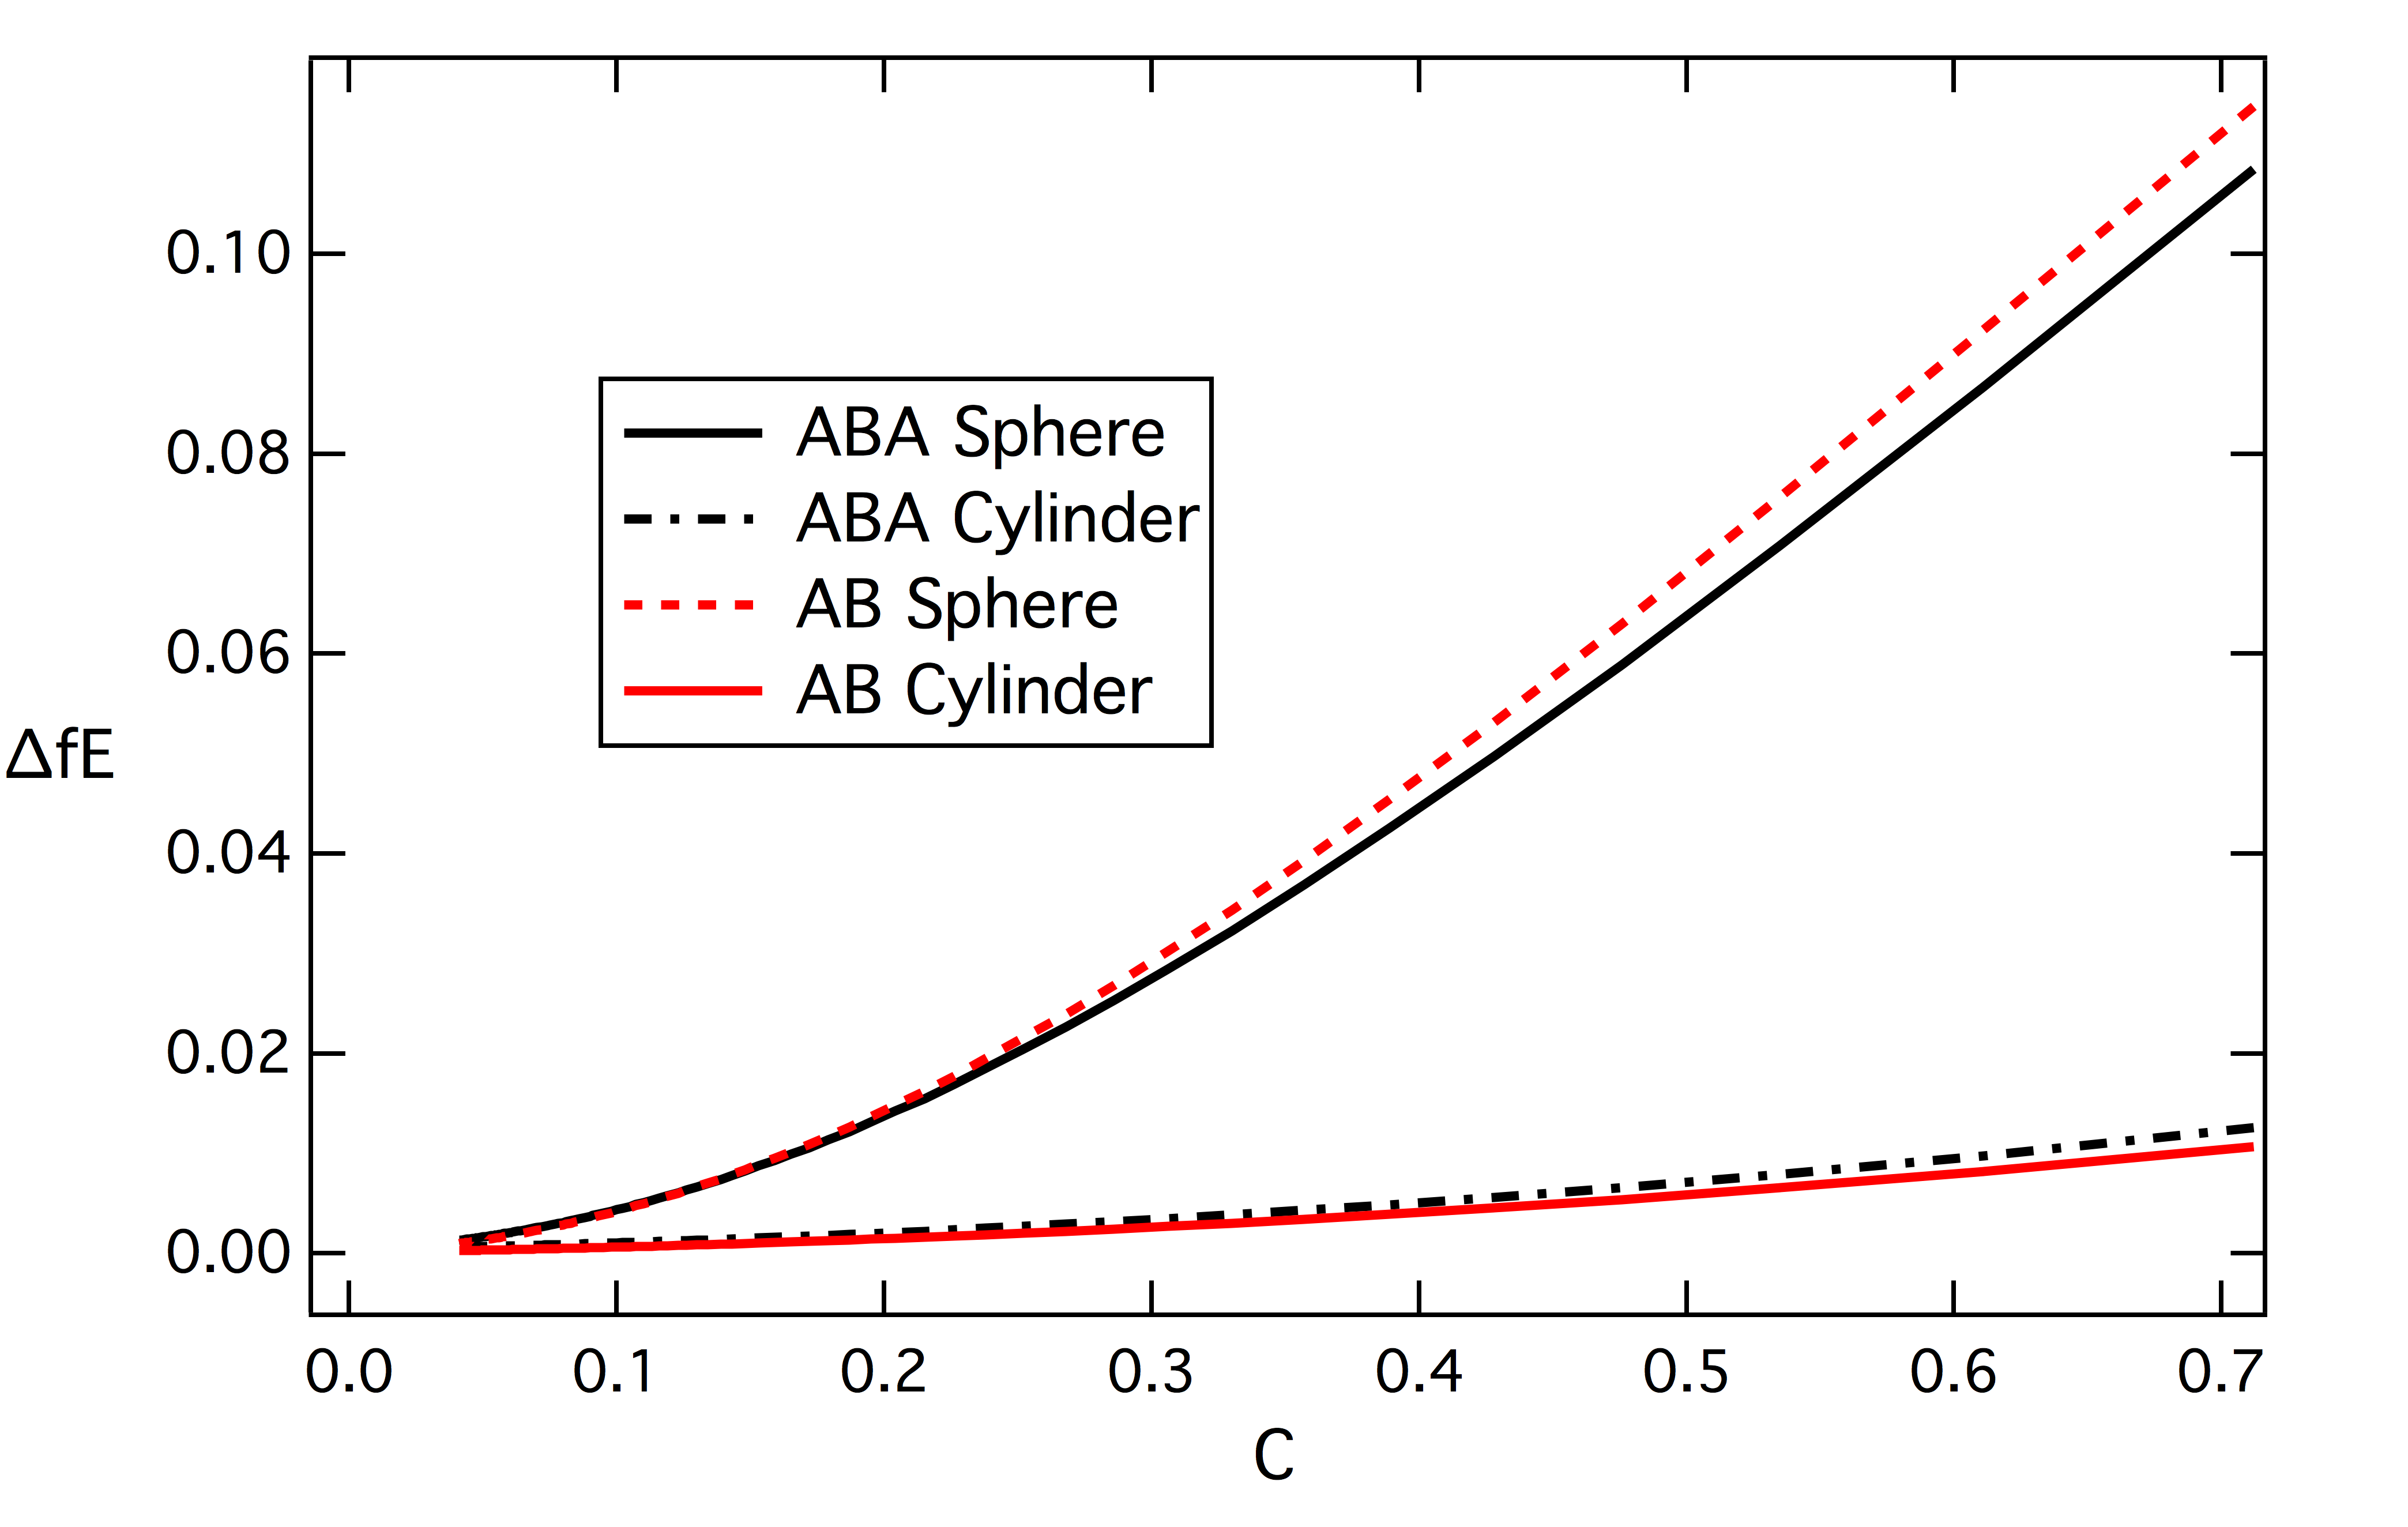
\includegraphics[scale=0.6]{BendingdfE}
\centering
\end{figure}

In order to determine the Mean and Gaussian bending moduli, the first step is to calculate the Mean bending moduli from the cylindrical geometries using a curve fitting algorithm. For the second order bending moduli, I restricted the fit to a region of lower curvature ($c=0...0.5$). The calculated bending moduli are in Table XX.

\begin{table}[H]
\centering
\begin{center}
\begin{tabular}[c]{| c | c | c |}
\hline
Architecture &$\kappa_M$ (Units) &Fit std. dev. \\
\hline
AB 	&0.0599 &$\pm$0.001\\
ABA	&0.0669 &$\pm$-20.0007 \\
\hline
\end{tabular}
\end{center}
\caption{\small{Mean bending modulus calculation}}
\end{table}

Using the mean curvature bending modulus, we can then determine the Gaussian bending modulus. This is shown in Table XX.

\begin{table}[H]
\centering
\begin{center}
\begin{tabular}[c]{| c | c | c |}
\hline
Architecture &$\kappa_G$ (Units) &Fit std. dev. \\
\hline
AB 	&0.240 &$\pm$0.002 \\
ABA	&0.206 &$\pm$0.003\\
\hline
\end{tabular}
\end{center}
\caption{\small{Gaussian bending modulus calculation}}
\end{table}

\section{Fourth order bending moduli}

At high curvatures, we require fourth order bending moduli to account for the change in Free energy. In the cylindrical coordinate system, we have a free energy $F^C$ of the form:

\begin{equation}
F^C = \frac{\kappa_M}{2} C^2 + B_C C^4
\end{equation}

Where $B_C$ is a coefficient that encompasses all fourth order curvature terms into what we will call the cylindrical fourth order bending modulus.

In the spherical coordinate system, we have a free energy $F^S$ of the form:

\begin{equation}
F^S = (2 \kappa_M + \kappa_G)C^2 + B_S C^4
\end{equation}

Where $B_S$ is a coefficient that encompasses all fourth order curvature terms into what we will call the spherical fourth order bending modulus.

The results are shown in Figure XX.

\begin{table}[H]
\centering
\begin{center}
\begin{tabular}[c]{| c | c | c | c | c |}
\hline
Architecture &$B_C$ (Units) &Fit std. dev. &$B_S$ &Fit std. dev. \\
\hline
AB 	&-0.0037 & $\pm$0.002 &-0.137 &$\pm$0.005\\
ABA	&-0.0031 & $\pm$0.001 &-0.126 &$\pm$0.006\\
\hline
\end{tabular}
\end{center}
\caption{\small{Gaussian bending modulus calculation}}
\end{table}

There were a number of inconsistencies in these calculations, and the free energy curves didn't fit particularly well. It was discovered that there was an error in the homogeneous free energy calculation, so the results may be entirely wrong. However, this was good practice for practicing the method I'll be using to determine the bending moduli for the two types of membranes.


\section{Testing $\chi$ dependence}

There was an issue with the homogeneous free energy calculation, and the free energy didn't match my homogeneous free energy calculation (homogfE) when the interaction parameter was set such that the system was in a disordered state. This is obviously wrong, and I eventually fixed the mistake. To ensure that the mistake was fixed, I calculated the free energy of the AB diblock and ABA triblock systems as they transitioned from the lamellar state to the disordered state. The expectation is that the difference between fE and homogfE (typically denoted $\Delta fE$) should reach zero at specfic $\chi_AB$ that correspond to the location of the phase transition between lamellar and disorder. The results from the calculation are shown in Figure XX.

\begin{figure}[H]
\centering
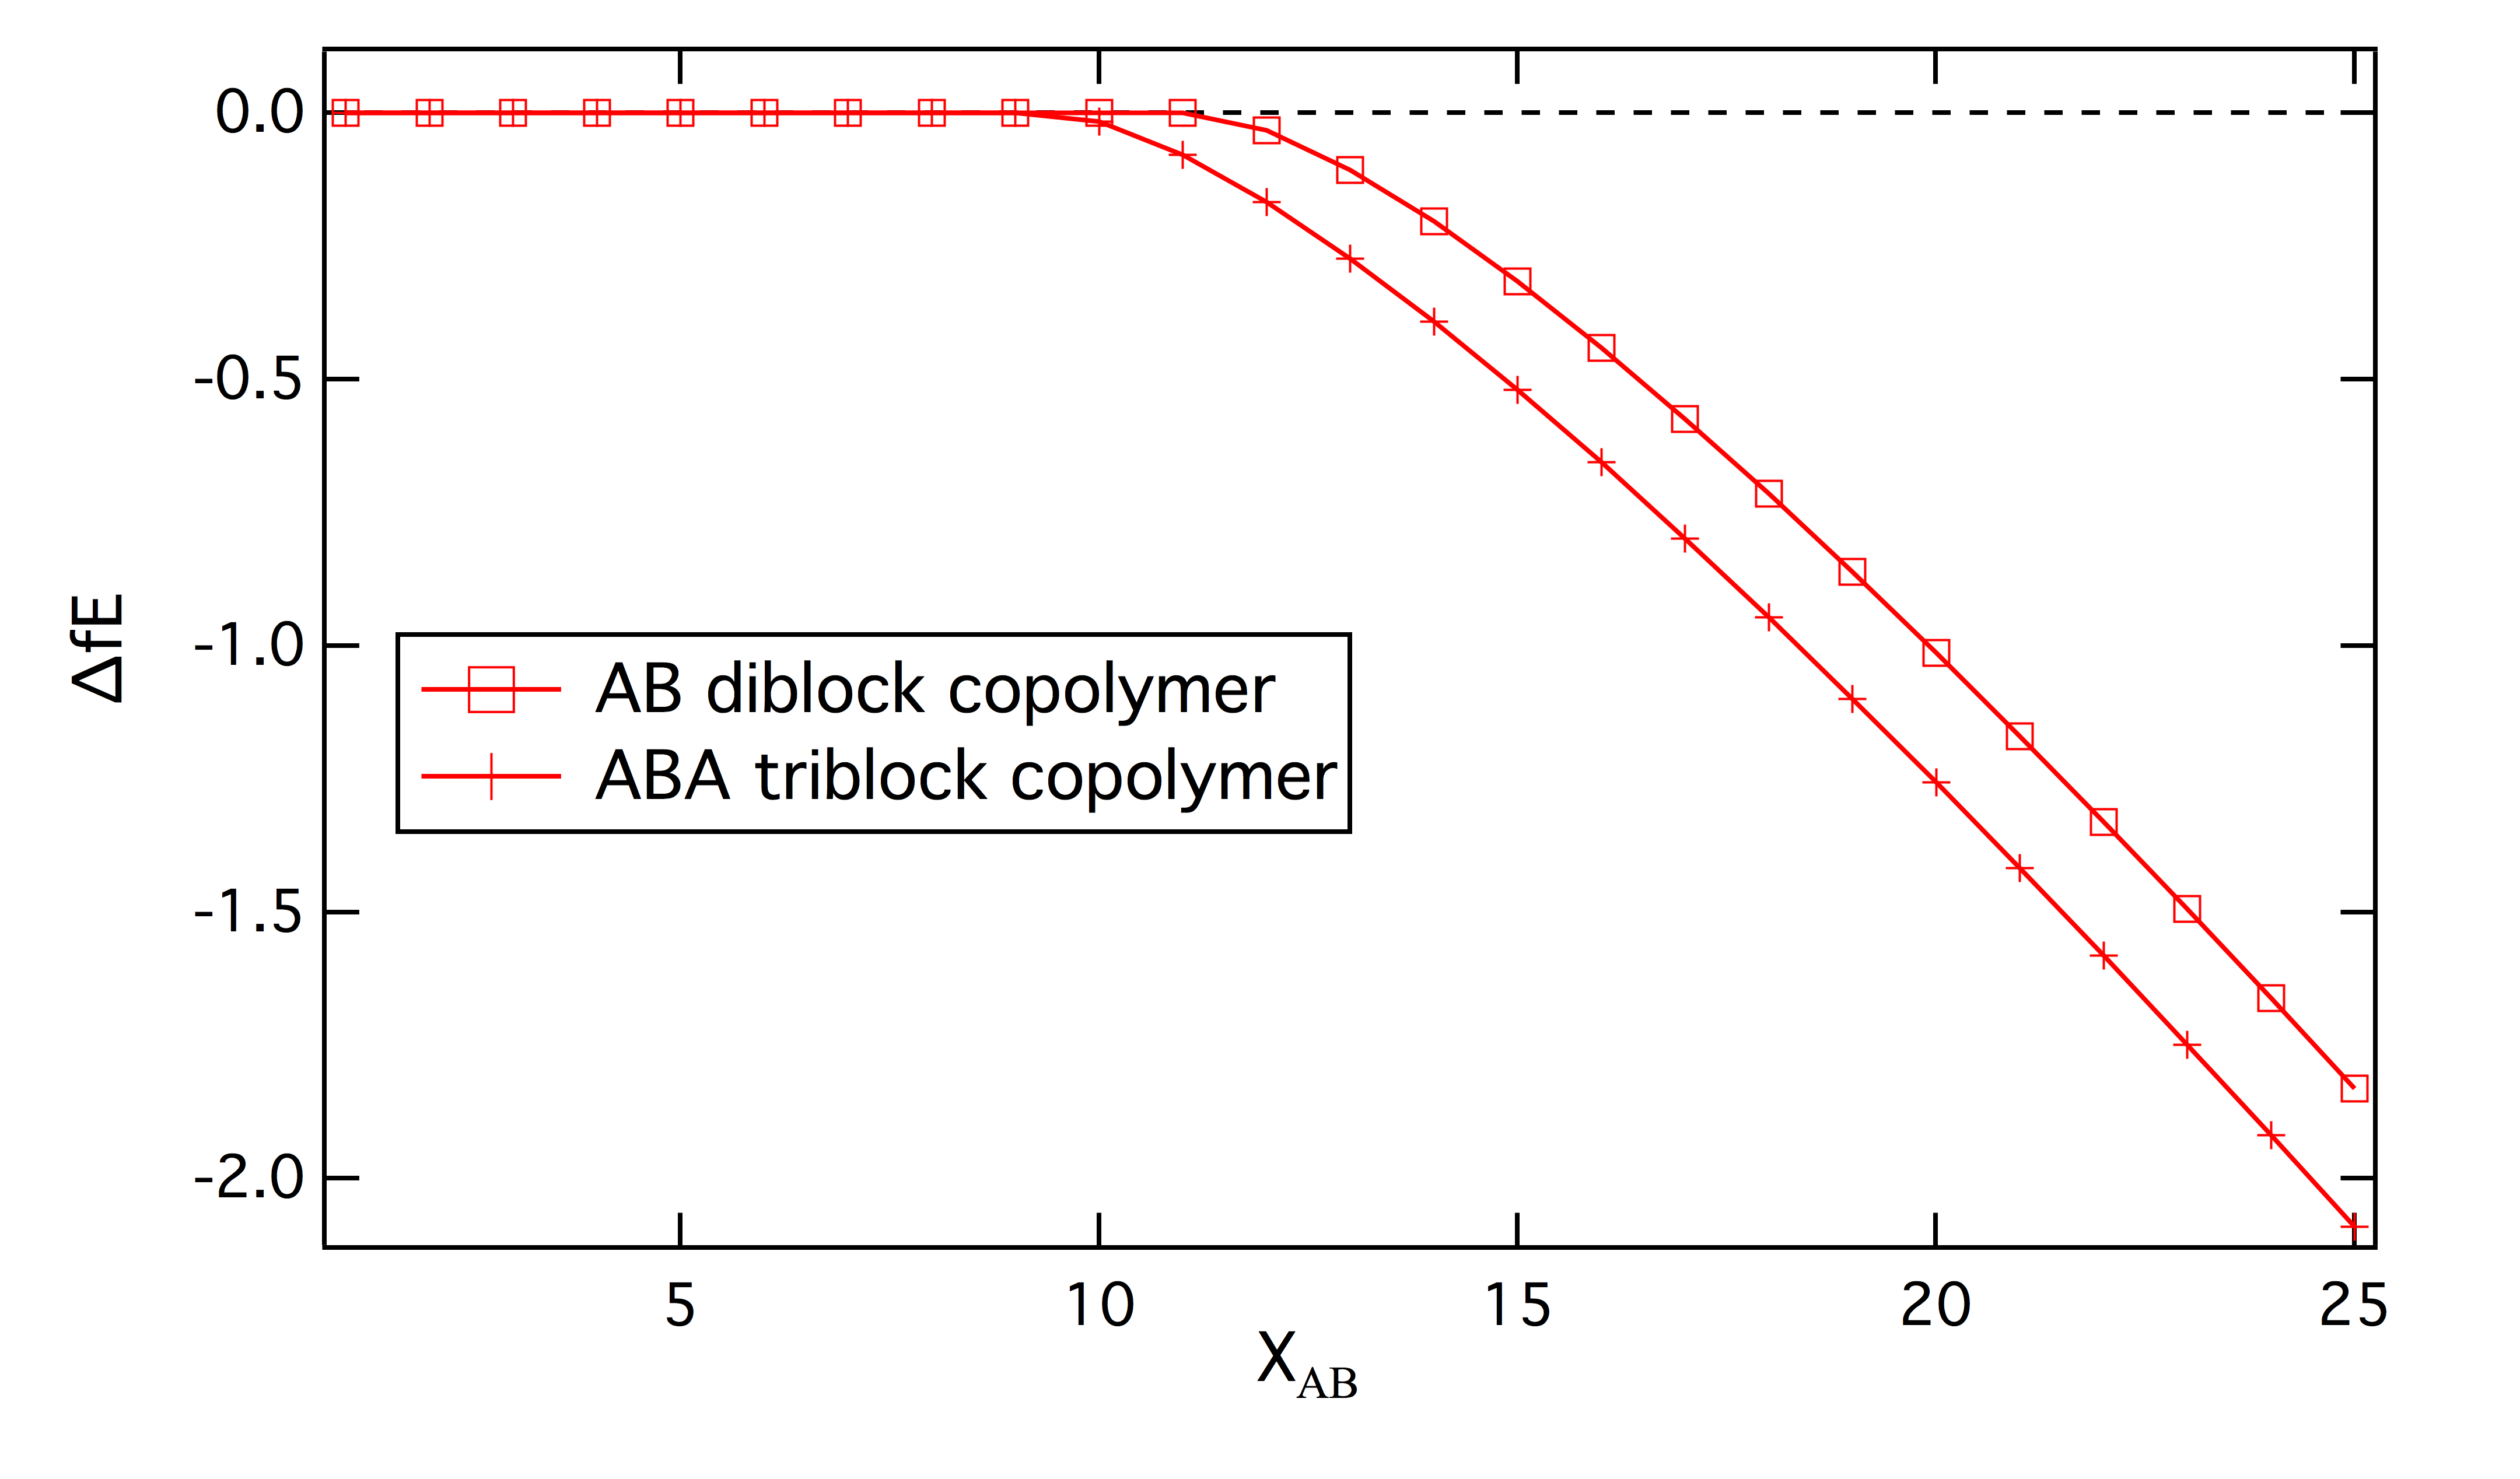
\includegraphics[scale=0.7]{chi_conv}
\centering
\end{figure}


\end{document}